\documentclass[1p]{elsarticle_modified}
%\bibliographystyle{elsarticle-num}

%\usepackage[colorlinks]{hyperref}
%\usepackage{abbrmath_seonhwa} %\Abb, \Ascr, \Acal ,\Abf, \Afrak
\usepackage{amsfonts}
\usepackage{amssymb}
\usepackage{amsmath}
\usepackage{amsthm}
\usepackage{scalefnt}
\usepackage{amsbsy}
\usepackage{kotex}
\usepackage{caption}
\usepackage{subfig}
\usepackage{color}
\usepackage{graphicx}
\usepackage{xcolor} %% white, black, red, green, blue, cyan, magenta, yellow
\usepackage{float}
\usepackage{setspace}
\usepackage{hyperref}

\usepackage{tikz}
\usetikzlibrary{arrows}

\usepackage{multirow}
\usepackage{array} % fixed length table
\usepackage{hhline}

%%%%%%%%%%%%%%%%%%%%%
\makeatletter
\renewcommand*\env@matrix[1][\arraystretch]{%
	\edef\arraystretch{#1}%
	\hskip -\arraycolsep
	\let\@ifnextchar\new@ifnextchar
	\array{*\c@MaxMatrixCols c}}
\makeatother %https://tex.stackexchange.com/questions/14071/how-can-i-increase-the-line-spacing-in-a-matrix
%%%%%%%%%%%%%%%

\usepackage[normalem]{ulem}

\newcommand{\msout}[1]{\ifmmode\text{\sout{\ensuremath{#1}}}\else\sout{#1}\fi}
%SOURCE: \msout is \stkout macro in https://tex.stackexchange.com/questions/20609/strikeout-in-math-mode

\newcommand{\cancel}[1]{
	\ifmmode
	{\color{red}\msout{#1}}
	\else
	{\color{red}\sout{#1}}
	\fi
}

\newcommand{\add}[1]{
	{\color{blue}\uwave{#1}}
}

\newcommand{\replace}[2]{
	\ifmmode
	{\color{red}\msout{#1}}{\color{blue}\uwave{#2}}
	\else
	{\color{red}\sout{#1}}{\color{blue}\uwave{#2}}
	\fi
}

\newcommand{\Sol}{\mathcal{S}} %segment
\newcommand{\D}{D} %diagram
\newcommand{\A}{\mathcal{A}} %arc


%%%%%%%%%%%%%%%%%%%%%%%%%%%%%5 test

\def\sl{\operatorname{\textup{SL}}(2,\Cbb)}
\def\psl{\operatorname{\textup{PSL}}(2,\Cbb)}
\def\quan{\mkern 1mu \triangleright \mkern 1mu}

\theoremstyle{definition}
\newtheorem{thm}{Theorem}[section]
\newtheorem{prop}[thm]{Proposition}
\newtheorem{lem}[thm]{Lemma}
\newtheorem{ques}[thm]{Question}
\newtheorem{cor}[thm]{Corollary}
\newtheorem{defn}[thm]{Definition}
\newtheorem{exam}[thm]{Example}
\newtheorem{rmk}[thm]{Remark}
\newtheorem{alg}[thm]{Algorithm}

\newcommand{\I}{\sqrt{-1}}
\begin{document}

%\begin{frontmatter}
%
%\title{Boundary parabolic representations of knots up to 8 crossings}
%
%%% Group authors per affiliation:
%\author{Yunhi Cho} 
%\address{Department of Mathematics, University of Seoul, Seoul, Korea}
%\ead{yhcho@uos.ac.kr}
%
%
%\author{Seonhwa Kim} %\fnref{s_kim}}
%\address{Center for Geometry and Physics, Institute for Basic Science, Pohang, 37673, Korea}
%\ead{ryeona17@ibs.re.kr}
%
%\author{Hyuk Kim}
%\address{Department of Mathematical Sciences, Seoul National University, Seoul 08826, Korea}
%\ead{hyukkim@snu.ac.kr}
%
%\author{Seokbeom Yoon}
%\address{Department of Mathematical Sciences, Seoul National University, Seoul, 08826,  Korea}
%\ead{sbyoon15@snu.ac.kr}
%
%\begin{abstract}
%We find all boundary parabolic representation of knots up to 8 crossings.
%
%\end{abstract}
%\begin{keyword}
%    \MSC[2010] 57M25 
%\end{keyword}
%
%\end{frontmatter}

%\linenumbers
%\tableofcontents
%
\newcommand\colored[1]{\textcolor{white}{\rule[-0.35ex]{0.8em}{1.4ex}}\kern-0.8em\color{red} #1}%
%\newcommand\colored[1]{\textcolor{white}{ #1}\kern-2.17ex	\textcolor{white}{ #1}\kern-1.81ex	\textcolor{white}{ #1}\kern-2.15ex\color{red}#1	}

{\Large $\underline{12n_{0284}~(K12n_{0284})}$}

\setlength{\tabcolsep}{10pt}
\renewcommand{\arraystretch}{1.6}
\vspace{1cm}\begin{tabular}{m{100pt}>{\centering\arraybackslash}m{274pt}}
\multirow{5}{120pt}{
	\centering
	\includegraphics[width=112pt]{../../../GIT/diagram.site/Diagrams/png/2373_12n_0284.png}\\
\ \ \ A knot diagram\footnotemark}&
\allowdisplaybreaks
\textbf{Linearized knot diagam} \\
\cline{2-2}
 &
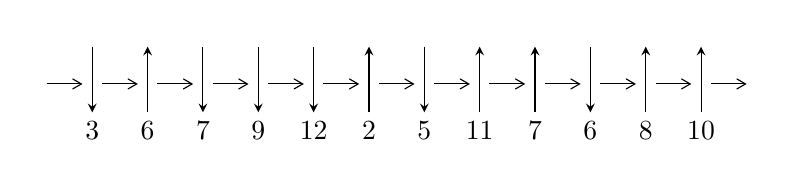
\begin{tikzpicture}[x=20pt, y=17pt]
	% nodes
	\node (C0) at (0, 0) {};
	\node (C1) at (1, 0) {};
	\node (C1U) at (1, +1) {};
	\node (C1D) at (1, -1) {3};

	\node (C2) at (2, 0) {};
	\node (C2U) at (2, +1) {};
	\node (C2D) at (2, -1) {6};

	\node (C3) at (3, 0) {};
	\node (C3U) at (3, +1) {};
	\node (C3D) at (3, -1) {7};

	\node (C4) at (4, 0) {};
	\node (C4U) at (4, +1) {};
	\node (C4D) at (4, -1) {9};

	\node (C5) at (5, 0) {};
	\node (C5U) at (5, +1) {};
	\node (C5D) at (5, -1) {12};

	\node (C6) at (6, 0) {};
	\node (C6U) at (6, +1) {};
	\node (C6D) at (6, -1) {2};

	\node (C7) at (7, 0) {};
	\node (C7U) at (7, +1) {};
	\node (C7D) at (7, -1) {5};

	\node (C8) at (8, 0) {};
	\node (C8U) at (8, +1) {};
	\node (C8D) at (8, -1) {11};

	\node (C9) at (9, 0) {};
	\node (C9U) at (9, +1) {};
	\node (C9D) at (9, -1) {7};

	\node (C10) at (10, 0) {};
	\node (C10U) at (10, +1) {};
	\node (C10D) at (10, -1) {6};

	\node (C11) at (11, 0) {};
	\node (C11U) at (11, +1) {};
	\node (C11D) at (11, -1) {8};

	\node (C12) at (12, 0) {};
	\node (C12U) at (12, +1) {};
	\node (C12D) at (12, -1) {10};
	\node (C13) at (13, 0) {};

	% arrows
	\draw[->,>={angle 60}]
	(C0) edge (C1) (C1) edge (C2) (C2) edge (C3) (C3) edge (C4) (C4) edge (C5) (C5) edge (C6) (C6) edge (C7) (C7) edge (C8) (C8) edge (C9) (C9) edge (C10) (C10) edge (C11) (C11) edge (C12) (C12) edge (C13) ;	\draw[->,>=stealth]
	(C1U) edge (C1D) (C2D) edge (C2U) (C3U) edge (C3D) (C4U) edge (C4D) (C5U) edge (C5D) (C6D) edge (C6U) (C7U) edge (C7D) (C8D) edge (C8U) (C9D) edge (C9U) (C10U) edge (C10D) (C11D) edge (C11U) (C12D) edge (C12U) ;
	\end{tikzpicture} \\
\hhline{~~} \\& 
\textbf{Solving Sequence} \\ \cline{2-2} 
 &
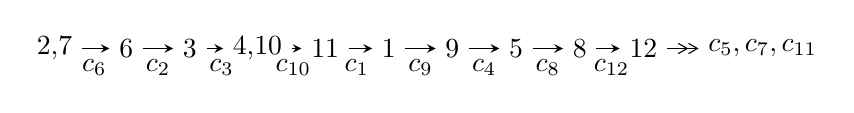
\begin{tikzpicture}[x=23pt, y=7pt]
	% node
	\node (A0) at (-1/8, 0) {2,7};
	\node (A1) at (1, 0) {6};
	\node (A2) at (2, 0) {3};
	\node (A3) at (49/16, 0) {4,10};
	\node (A4) at (33/8, 0) {11};
	\node (A5) at (41/8, 0) {1};
	\node (A6) at (49/8, 0) {9};
	\node (A7) at (57/8, 0) {5};
	\node (A8) at (65/8, 0) {8};
	\node (A9) at (73/8, 0) {12};
	\node (C1) at (1/2, -1) {$c_{6}$};
	\node (C2) at (3/2, -1) {$c_{2}$};
	\node (C3) at (5/2, -1) {$c_{3}$};
	\node (C4) at (29/8, -1) {$c_{10}$};
	\node (C5) at (37/8, -1) {$c_{1}$};
	\node (C6) at (45/8, -1) {$c_{9}$};
	\node (C7) at (53/8, -1) {$c_{4}$};
	\node (C8) at (61/8, -1) {$c_{8}$};
	\node (C9) at (69/8, -1) {$c_{12}$};
	\node (A10) at (11, 0) {$c_{5},c_{7},c_{11}$};

	% edge
	\draw[->,>=stealth]	
	(A0) edge (A1) (A1) edge (A2) (A2) edge (A3) (A3) edge (A4) (A4) edge (A5) (A5) edge (A6) (A6) edge (A7) (A7) edge (A8) (A8) edge (A9) ;
	\draw[->>,>={angle 60}]	
	(A9) edge (A10);
\end{tikzpicture} \\ 

\end{tabular} \\

\footnotetext{
The image of knot diagram is generated by the software ``\textbf{Draw programme}" developed by Andrew Bartholomew(\url{http://www.layer8.co.uk/maths/draw/index.htm\#Running-draw}), where we modified some parts for our purpose(\url{https://github.com/CATsTAILs/LinksPainter}).
}\phantom \\ \newline 
\centering \textbf{Ideals for irreducible components\footnotemark of $X_{\text{par}}$} 
 
\begin{align*}
I^u_{1}&=\langle 
-157641 u^{22}+1055893 u^{21}+\cdots+43337 b+207103,\\
\phantom{I^u_{1}}&\phantom{= \langle  }27883 u^{22}-413880 u^{21}+\cdots+86674 a-184081,\;u^{23}-8 u^{22}+\cdots-11 u+2\rangle \\
I^u_{2}&=\langle 
u^8+3 u^7+6 u^6+7 u^5+6 u^4+3 u^3+u^2+b-1,\\
\phantom{I^u_{2}}&\phantom{= \langle  }- u^{12}-6 u^{11}-19 u^{10}-40 u^9-61 u^8-70 u^7-60 u^6-37 u^5-12 u^4+5 u^3+10 u^2+a+8 u+3,\\
\phantom{I^u_{2}}&\phantom{= \langle  }u^{13}+5 u^{12}+15 u^{11}+30 u^{10}+45 u^9+51 u^8+45 u^7+30 u^6+13 u^5+u^4-5 u^3-5 u^2-2 u-1\rangle \\
I^u_{3}&=\langle 
2 u^{12} a+29 u^{12}+\cdots+2 a+35,\;5 u^{12} a+9 u^{12}+\cdots+3 a+18,\\
\phantom{I^u_{3}}&\phantom{= \langle  }u^{13}+3 u^{12}+5 u^{11}+4 u^{10}+4 u^9+3 u^8+u^7-4 u^6-2 u^5+u^3+3 u^2+3 u+1\rangle \\
I^u_{4}&=\langle 
a^3 u+a^3- a^2 u- a u+4 b-4 a-4 u+1,\;a^4+2 a^2 u-3 a^2-2 a u-2 a-1,\;u^2- u+1\rangle \\
\\
\end{align*}
\raggedright * 4 irreducible components of $\dim_{\mathbb{C}}=0$, with total 70 representations.\\
\footnotetext{All coefficients of polynomials are rational numbers. But the coefficients are sometimes approximated in decimal forms when there is not enough margin.}
\newpage
\renewcommand{\arraystretch}{1}
\centering \section*{I. $I^u_{1}= \langle -1.58\times10^{5} u^{22}+1.06\times10^{6} u^{21}+\cdots+4.33\times10^{4} b+2.07\times10^{5},\;27883 u^{22}-413880 u^{21}+\cdots+86674 a-184081,\;u^{23}-8 u^{22}+\cdots-11 u+2 \rangle$}
\flushleft \textbf{(i) Arc colorings}\\
\begin{tabular}{m{7pt} m{180pt} m{7pt} m{180pt} }
\flushright $a_{2}=$&$\begin{pmatrix}0\\u\end{pmatrix}$ \\
\flushright $a_{7}=$&$\begin{pmatrix}1\\0\end{pmatrix}$ \\
\flushright $a_{6}=$&$\begin{pmatrix}1\\u^2\end{pmatrix}$ \\
\flushright $a_{3}=$&$\begin{pmatrix}u\\u^3+u\end{pmatrix}$ \\
\flushright $a_{4}=$&$\begin{pmatrix}- u^3\\u^3+u\end{pmatrix}$ \\
\flushright $a_{10}=$&$\begin{pmatrix}-0.321700 u^{22}+4.77513 u^{21}+\cdots-26.2727 u+2.12383\\3.63756 u^{22}-24.3647 u^{21}+\cdots+24.4277 u-4.77890\end{pmatrix}$ \\
\flushright $a_{11}=$&$\begin{pmatrix}-0.187911 u^{22}+1.63708 u^{21}+\cdots-25.8401 u+2.49965\\-2.20154 u^{22}+13.8409 u^{21}+\cdots+1.41486 u-0.643399\end{pmatrix}$ \\
\flushright $a_{1}=$&$\begin{pmatrix}u^3\\u^5+u^3+u\end{pmatrix}$ \\
\flushright $a_{9}=$&$\begin{pmatrix}-3.95926 u^{22}+29.1398 u^{21}+\cdots-50.7004 u+6.90273\\3.63756 u^{22}-24.3647 u^{21}+\cdots+24.4277 u-4.77890\end{pmatrix}$ \\
\flushright $a_{5}=$&$\begin{pmatrix}1.25086 u^{22}-9.29017 u^{21}+\cdots-1.10816 u+6.18493\\-1.69428 u^{22}+12.2032 u^{21}+\cdots-15.3776 u+1.78376\end{pmatrix}$ \\
\flushright $a_{8}=$&$\begin{pmatrix}-1.06123 u^{22}+8.07276 u^{21}+\cdots-14.7681 u-3.81472\\0.492097 u^{22}-5.85550 u^{21}+\cdots+20.7596 u-3.21718\end{pmatrix}$ \\
\flushright $a_{12}=$&$\begin{pmatrix}-0.802397 u^{22}+6.76237 u^{21}+\cdots-26.6681 u+8.35061\\-0.134366 u^{22}+2.76904 u^{21}+\cdots-9.99762 u+1.09738\end{pmatrix}$\\&\end{tabular}
\flushleft \textbf{(ii) Obstruction class $= -1$}\\~\\
\flushleft \textbf{(iii) Cusp Shapes $= -\frac{52973}{43337} u^{22}+\frac{121642}{43337} u^{21}+\cdots+\frac{1232071}{43337} u-\frac{582900}{43337}$}\\~\\
\newpage\renewcommand{\arraystretch}{1}
\flushleft \textbf{(iv) u-Polynomials at the component}\newline \\
\begin{tabular}{m{50pt}|m{274pt}}
Crossings & \hspace{64pt}u-Polynomials at each crossing \\
\hline $$\begin{aligned}c_{1}\end{aligned}$$&$\begin{aligned}
&u^{23}+4 u^{22}+\cdots-35 u-4
\end{aligned}$\\
\hline $$\begin{aligned}c_{2},c_{6}\end{aligned}$$&$\begin{aligned}
&u^{23}-8 u^{22}+\cdots-11 u+2
\end{aligned}$\\
\hline $$\begin{aligned}c_{3}\end{aligned}$$&$\begin{aligned}
&u^{23}+8 u^{22}+\cdots-17339 u+16754
\end{aligned}$\\
\hline $$\begin{aligned}c_{4},c_{10}\end{aligned}$$&$\begin{aligned}
&u^{23}+16 u^{21}+\cdots-4 u-1
\end{aligned}$\\
\hline $$\begin{aligned}c_{5},c_{7}\end{aligned}$$&$\begin{aligned}
&u^{23}-8 u^{21}+\cdots+5 u-1
\end{aligned}$\\
\hline $$\begin{aligned}c_{8},c_{11}\end{aligned}$$&$\begin{aligned}
&u^{23}+10 u^{22}+\cdots-29 u-4
\end{aligned}$\\
\hline $$\begin{aligned}c_{9},c_{12}\end{aligned}$$&$\begin{aligned}
&u^{23}+3 u^{22}+\cdots-10 u-1
\end{aligned}$\\
\hline
\end{tabular}\\~\\
\newpage\renewcommand{\arraystretch}{1}
\flushleft \textbf{(v) Riley Polynomials at the component}\newline \\
\begin{tabular}{m{50pt}|m{274pt}}
Crossings & \hspace{64pt}Riley Polynomials at each crossing \\
\hline $$\begin{aligned}c_{1}\end{aligned}$$&$\begin{aligned}
&y^{23}+44 y^{22}+\cdots-1519 y-16
\end{aligned}$\\
\hline $$\begin{aligned}c_{2},c_{6}\end{aligned}$$&$\begin{aligned}
&y^{23}+4 y^{22}+\cdots-35 y-4
\end{aligned}$\\
\hline $$\begin{aligned}c_{3}\end{aligned}$$&$\begin{aligned}
&y^{23}+84 y^{22}+\cdots-4785303843 y-280696516
\end{aligned}$\\
\hline $$\begin{aligned}c_{4},c_{10}\end{aligned}$$&$\begin{aligned}
&y^{23}+32 y^{22}+\cdots+2 y-1
\end{aligned}$\\
\hline $$\begin{aligned}c_{5},c_{7}\end{aligned}$$&$\begin{aligned}
&y^{23}-16 y^{22}+\cdots+33 y-1
\end{aligned}$\\
\hline $$\begin{aligned}c_{8},c_{11}\end{aligned}$$&$\begin{aligned}
&y^{23}+6 y^{22}+\cdots-575 y-16
\end{aligned}$\\
\hline $$\begin{aligned}c_{9},c_{12}\end{aligned}$$&$\begin{aligned}
&y^{23}-39 y^{22}+\cdots-196 y-1
\end{aligned}$\\
\hline
\end{tabular}\\~\\
\newpage\flushleft \textbf{(vi) Complex Volumes and Cusp Shapes}
$$\begin{array}{c|c|c}  
\text{Solutions to }I^u_{1}& \I (\text{vol} + \sqrt{-1}CS) & \text{Cusp shape}\\
 \hline 
\begin{aligned}
u &= \phantom{-}0.482213 + 0.920645 I \\
a &= \phantom{-}0.244578 - 0.919306 I \\
b &= \phantom{-}0.0382942 + 0.0881044 I\end{aligned}
 & -1.61303 + 2.07315 I & -0.31329 - 3.51886 I \\ \hline\begin{aligned}
u &= \phantom{-}0.482213 - 0.920645 I \\
a &= \phantom{-}0.244578 + 0.919306 I \\
b &= \phantom{-}0.0382942 - 0.0881044 I\end{aligned}
 & -1.61303 - 2.07315 I & -0.31329 + 3.51886 I \\ \hline\begin{aligned}
u &= \phantom{-}0.795198 + 0.518466 I \\
a &= \phantom{-}0.729958 + 0.210265 I \\
b &= \phantom{-}0.691674 - 0.467858 I\end{aligned}
 & -0.22104 + 2.41394 I & \phantom{-}1.23274 - 2.49732 I \\ \hline\begin{aligned}
u &= \phantom{-}0.795198 - 0.518466 I \\
a &= \phantom{-}0.729958 - 0.210265 I \\
b &= \phantom{-}0.691674 + 0.467858 I\end{aligned}
 & -0.22104 - 2.41394 I & \phantom{-}1.23274 + 2.49732 I \\ \hline\begin{aligned}
u &= -0.400101 + 1.050250 I \\
a &= \phantom{-}0.662095 + 0.548805 I \\
b &= \phantom{-}0.384543 - 1.002950 I\end{aligned}
 & -6.34034 - 1.70564 I & -9.62352 + 2.67791 I \\ \hline\begin{aligned}
u &= -0.400101 - 1.050250 I \\
a &= \phantom{-}0.662095 - 0.548805 I \\
b &= \phantom{-}0.384543 + 1.002950 I\end{aligned}
 & -6.34034 + 1.70564 I & -9.62352 - 2.67791 I \\ \hline\begin{aligned}
u &= -0.787767 + 0.322879 I \\
a &= \phantom{-}0.846615 - 0.478402 I \\
b &= \phantom{-}0.534974 - 0.979772 I\end{aligned}
 & -2.52532 + 1.25135 I & -2.51529 - 0.59191 I \\ \hline\begin{aligned}
u &= -0.787767 - 0.322879 I \\
a &= \phantom{-}0.846615 + 0.478402 I \\
b &= \phantom{-}0.534974 + 0.979772 I\end{aligned}
 & -2.52532 - 1.25135 I & -2.51529 + 0.59191 I \\ \hline\begin{aligned}
u &= \phantom{-}0.274775 + 0.733362 I \\
a &= \phantom{-}0.596051 + 0.164908 I \\
b &= -0.038646 - 0.194454 I\end{aligned}
 & -0.352945 + 1.192290 I & -4.51268 - 5.42631 I \\ \hline\begin{aligned}
u &= \phantom{-}0.274775 - 0.733362 I \\
a &= \phantom{-}0.596051 - 0.164908 I \\
b &= -0.038646 + 0.194454 I\end{aligned}
 & -0.352945 - 1.192290 I & -4.51268 + 5.42631 I\\
 \hline 
 \end{array}$$\newpage$$\begin{array}{c|c|c}  
\text{Solutions to }I^u_{1}& \I (\text{vol} + \sqrt{-1}CS) & \text{Cusp shape}\\
 \hline 
\begin{aligned}
u &= -0.555047 + 1.233680 I \\
a &= -0.578619 + 0.250416 I \\
b &= \phantom{-}0.773467 + 0.821194 I\end{aligned}
 & -5.25580 - 6.48914 I & -3.11761 + 2.59067 I \\ \hline\begin{aligned}
u &= -0.555047 - 1.233680 I \\
a &= -0.578619 - 0.250416 I \\
b &= \phantom{-}0.773467 - 0.821194 I\end{aligned}
 & -5.25580 + 6.48914 I & -3.11761 - 2.59067 I \\ \hline\begin{aligned}
u &= -0.646784\phantom{ +0.000000I} \\
a &= -1.86113\phantom{ +0.000000I} \\
b &= -1.50954\phantom{ +0.000000I}\end{aligned}
 & \phantom{-}2.52927\phantom{ +0.000000I} & \phantom{-}13.5670\phantom{ +0.000000I} \\ \hline\begin{aligned}
u &= \phantom{-}1.13690 + 0.99514 I \\
a &= \phantom{-}0.847752 - 0.965637 I \\
b &= \phantom{-}2.45166 - 0.30632 I\end{aligned}
 & \phantom{-}8.67002 - 6.60337 I & \phantom{-}0.16824 + 3.17637 I \\ \hline\begin{aligned}
u &= \phantom{-}1.13690 - 0.99514 I \\
a &= \phantom{-}0.847752 + 0.965637 I \\
b &= \phantom{-}2.45166 + 0.30632 I\end{aligned}
 & \phantom{-}8.67002 + 6.60337 I & \phantom{-}0.16824 - 3.17637 I \\ \hline\begin{aligned}
u &= \phantom{-}1.02850 + 1.11001 I \\
a &= \phantom{-}1.24376 - 0.88643 I \\
b &= \phantom{-}2.28163 + 0.96771 I\end{aligned}
 & \phantom{-}8.2361 + 14.4853 I & -0.53177 - 7.04602 I \\ \hline\begin{aligned}
u &= \phantom{-}1.02850 - 1.11001 I \\
a &= \phantom{-}1.24376 + 0.88643 I \\
b &= \phantom{-}2.28163 - 0.96771 I\end{aligned}
 & \phantom{-}8.2361 - 14.4853 I & -0.53177 + 7.04602 I \\ \hline\begin{aligned}
u &= \phantom{-}1.13613 + 1.00401 I \\
a &= -1.060840 + 0.748303 I \\
b &= -2.47675 - 0.32354 I\end{aligned}
 & \phantom{-}10.85390 + 6.57430 I & \phantom{-}0.18173 - 4.98395 I \\ \hline\begin{aligned}
u &= \phantom{-}1.13613 - 1.00401 I \\
a &= -1.060840 - 0.748303 I \\
b &= -2.47675 + 0.32354 I\end{aligned}
 & \phantom{-}10.85390 - 6.57430 I & \phantom{-}0.18173 + 4.98395 I \\ \hline\begin{aligned}
u &= \phantom{-}1.04311 + 1.14169 I \\
a &= -0.869736 + 0.998294 I \\
b &= -2.21575 - 0.49458 I\end{aligned}
 & \phantom{-}10.38880 + 1.40736 I & -0.548351 + 0.550968 I\\
 \hline 
 \end{array}$$\newpage$$\begin{array}{c|c|c}  
\text{Solutions to }I^u_{1}& \I (\text{vol} + \sqrt{-1}CS) & \text{Cusp shape}\\
 \hline 
\begin{aligned}
u &= \phantom{-}1.04311 - 1.14169 I \\
a &= -0.869736 - 0.998294 I \\
b &= -2.21575 + 0.49458 I\end{aligned}
 & \phantom{-}10.38880 - 1.40736 I & -0.548351 - 0.550968 I \\ \hline\begin{aligned}
u &= \phantom{-}0.169482 + 0.280800 I \\
a &= -2.98105 - 2.07240 I \\
b &= -0.170327 + 1.076150 I\end{aligned}
 & -3.36571 + 0.11521 I & -6.20379 + 0.79398 I \\ \hline\begin{aligned}
u &= \phantom{-}0.169482 - 0.280800 I \\
a &= -2.98105 + 2.07240 I \\
b &= -0.170327 - 1.076150 I\end{aligned}
 & -3.36571 - 0.11521 I & -6.20379 - 0.79398 I\\
 \hline 
 \end{array}$$\newpage\newpage\renewcommand{\arraystretch}{1}
\centering \section*{II. $I^u_{2}= \langle u^8+3 u^7+6 u^6+7 u^5+6 u^4+3 u^3+u^2+b-1,\;- u^{12}-6 u^{11}+\cdots+a+3,\;u^{13}+5 u^{12}+\cdots-2 u-1 \rangle$}
\flushleft \textbf{(i) Arc colorings}\\
\begin{tabular}{m{7pt} m{180pt} m{7pt} m{180pt} }
\flushright $a_{2}=$&$\begin{pmatrix}0\\u\end{pmatrix}$ \\
\flushright $a_{7}=$&$\begin{pmatrix}1\\0\end{pmatrix}$ \\
\flushright $a_{6}=$&$\begin{pmatrix}1\\u^2\end{pmatrix}$ \\
\flushright $a_{3}=$&$\begin{pmatrix}u\\u^3+u\end{pmatrix}$ \\
\flushright $a_{4}=$&$\begin{pmatrix}- u^3\\u^3+u\end{pmatrix}$ \\
\flushright $a_{10}=$&$\begin{pmatrix}u^{12}+6 u^{11}+\cdots-8 u-3\\- u^8-3 u^7-6 u^6-7 u^5-6 u^4-3 u^3- u^2+1\end{pmatrix}$ \\
\flushright $a_{11}=$&$\begin{pmatrix}u^{11}+5 u^{10}+14 u^9+26 u^8+35 u^7+35 u^6+25 u^5+12 u^4-5 u^2-5 u-3\\u^{12}+4 u^{11}+\cdots- u+1\end{pmatrix}$ \\
\flushright $a_{1}=$&$\begin{pmatrix}u^3\\u^5+u^3+u\end{pmatrix}$ \\
\flushright $a_{9}=$&$\begin{pmatrix}u^{12}+6 u^{11}+\cdots-8 u-4\\- u^8-3 u^7-6 u^6-7 u^5-6 u^4-3 u^3- u^2+1\end{pmatrix}$ \\
\flushright $a_{5}=$&$\begin{pmatrix}u^{12}+4 u^{11}+\cdots+3 u+3\\- u^{12}-5 u^{11}+\cdots+4 u^2+3 u\end{pmatrix}$ \\
\flushright $a_{8}=$&$\begin{pmatrix}- u^{12}-4 u^{11}+\cdots+u-2\\u^{11}+5 u^{10}+14 u^9+25 u^8+32 u^7+29 u^6+19 u^5+8 u^4-4 u^2-4 u-1\end{pmatrix}$ \\
\flushright $a_{12}=$&$\begin{pmatrix}- u^{12}-6 u^{11}+\cdots+6 u+2\\- u^4- u^3- u^2-1\end{pmatrix}$\\&\end{tabular}
\flushleft \textbf{(ii) Obstruction class $= 1$}\\~\\
\flushleft \textbf{(iii) Cusp Shapes $= - u^{12}+u^{11}+12 u^{10}+42 u^9+79 u^8+107 u^7+101 u^6+71 u^5+29 u^4-8 u^3-24 u^2-19 u-11$}\\~\\
\newpage\renewcommand{\arraystretch}{1}
\flushleft \textbf{(iv) u-Polynomials at the component}\newline \\
\begin{tabular}{m{50pt}|m{274pt}}
Crossings & \hspace{64pt}u-Polynomials at each crossing \\
\hline $$\begin{aligned}c_{1}\end{aligned}$$&$\begin{aligned}
&u^{13}-5 u^{12}+\cdots-6 u+1
\end{aligned}$\\
\hline $$\begin{aligned}c_{2}\end{aligned}$$&$\begin{aligned}
&u^{13}-5 u^{12}+\cdots-2 u+1
\end{aligned}$\\
\hline $$\begin{aligned}c_{3}\end{aligned}$$&$\begin{aligned}
&u^{13}+5 u^{12}+\cdots+2 u+5
\end{aligned}$\\
\hline $$\begin{aligned}c_{4},c_{10}\end{aligned}$$&$\begin{aligned}
&u^{13}+5 u^{11}+\cdots+2 u-1
\end{aligned}$\\
\hline $$\begin{aligned}c_{5},c_{7}\end{aligned}$$&$\begin{aligned}
&u^{13}-3 u^{11}+\cdots+3 u+1
\end{aligned}$\\
\hline $$\begin{aligned}c_{6}\end{aligned}$$&$\begin{aligned}
&u^{13}+5 u^{12}+\cdots-2 u-1
\end{aligned}$\\
\hline $$\begin{aligned}c_{8}\end{aligned}$$&$\begin{aligned}
&u^{13}+7 u^{12}+\cdots+18 u+5
\end{aligned}$\\
\hline $$\begin{aligned}c_{9},c_{12}\end{aligned}$$&$\begin{aligned}
&u^{13}-3 u^{12}+\cdots-2 u-1
\end{aligned}$\\
\hline $$\begin{aligned}c_{11}\end{aligned}$$&$\begin{aligned}
&u^{13}-7 u^{12}+\cdots+18 u-5
\end{aligned}$\\
\hline
\end{tabular}\\~\\
\newpage\renewcommand{\arraystretch}{1}
\flushleft \textbf{(v) Riley Polynomials at the component}\newline \\
\begin{tabular}{m{50pt}|m{274pt}}
Crossings & \hspace{64pt}Riley Polynomials at each crossing \\
\hline $$\begin{aligned}c_{1}\end{aligned}$$&$\begin{aligned}
&y^{13}+5 y^{12}+\cdots+30 y-1
\end{aligned}$\\
\hline $$\begin{aligned}c_{2},c_{6}\end{aligned}$$&$\begin{aligned}
&y^{13}+5 y^{12}+\cdots-6 y-1
\end{aligned}$\\
\hline $$\begin{aligned}c_{3}\end{aligned}$$&$\begin{aligned}
&y^{13}+5 y^{12}+\cdots-336 y-25
\end{aligned}$\\
\hline $$\begin{aligned}c_{4},c_{10}\end{aligned}$$&$\begin{aligned}
&y^{13}+10 y^{12}+\cdots-8 y-1
\end{aligned}$\\
\hline $$\begin{aligned}c_{5},c_{7}\end{aligned}$$&$\begin{aligned}
&y^{13}-6 y^{12}+\cdots+3 y-1
\end{aligned}$\\
\hline $$\begin{aligned}c_{8},c_{11}\end{aligned}$$&$\begin{aligned}
&y^{13}+3 y^{12}+\cdots+124 y-25
\end{aligned}$\\
\hline $$\begin{aligned}c_{9},c_{12}\end{aligned}$$&$\begin{aligned}
&y^{13}-13 y^{12}+\cdots+6 y-1
\end{aligned}$\\
\hline
\end{tabular}\\~\\
\newpage\flushleft \textbf{(vi) Complex Volumes and Cusp Shapes}
$$\begin{array}{c|c|c}  
\text{Solutions to }I^u_{2}& \I (\text{vol} + \sqrt{-1}CS) & \text{Cusp shape}\\
 \hline 
\begin{aligned}
u &= -1.014650 + 0.255879 I \\
a &= \phantom{-}0.308979 - 0.014833 I \\
b &= \phantom{-}0.725825 + 1.010700 I\end{aligned}
 & -1.27099 - 3.82062 I & -1.40679 + 4.63835 I \\ \hline\begin{aligned}
u &= -1.014650 - 0.255879 I \\
a &= \phantom{-}0.308979 + 0.014833 I \\
b &= \phantom{-}0.725825 - 1.010700 I\end{aligned}
 & -1.27099 + 3.82062 I & -1.40679 - 4.63835 I \\ \hline\begin{aligned}
u &= \phantom{-}0.197297 + 0.861440 I \\
a &= \phantom{-}0.401352 + 0.826342 I \\
b &= -0.709820 + 0.085882 I\end{aligned}
 & \phantom{-}0.746919 + 0.991007 I & \phantom{-}3.49980 - 2.09278 I \\ \hline\begin{aligned}
u &= \phantom{-}0.197297 - 0.861440 I \\
a &= \phantom{-}0.401352 - 0.826342 I \\
b &= -0.709820 - 0.085882 I\end{aligned}
 & \phantom{-}0.746919 - 0.991007 I & \phantom{-}3.49980 + 2.09278 I \\ \hline\begin{aligned}
u &= -0.388828 + 1.189390 I \\
a &= -0.898954 - 0.065194 I \\
b &= \phantom{-}0.527148 + 0.273002 I\end{aligned}
 & -5.76976 - 7.61792 I & -6.66397 + 8.10409 I \\ \hline\begin{aligned}
u &= -0.388828 - 1.189390 I \\
a &= -0.898954 + 0.065194 I \\
b &= \phantom{-}0.527148 - 0.273002 I\end{aligned}
 & -5.76976 + 7.61792 I & -6.66397 - 8.10409 I \\ \hline\begin{aligned}
u &= -0.490814 + 1.270180 I \\
a &= \phantom{-}0.514001 + 0.677479 I \\
b &= \phantom{-}0.053980 - 0.728775 I\end{aligned}
 & -4.83122 - 1.66695 I & -3.23585 + 1.59270 I \\ \hline\begin{aligned}
u &= -0.490814 - 1.270180 I \\
a &= \phantom{-}0.514001 - 0.677479 I \\
b &= \phantom{-}0.053980 + 0.728775 I\end{aligned}
 & -4.83122 + 1.66695 I & -3.23585 - 1.59270 I \\ \hline\begin{aligned}
u &= \phantom{-}0.593865\phantom{ +0.000000I} \\
a &= -2.20766\phantom{ +0.000000I} \\
b &= -1.60115\phantom{ +0.000000I}\end{aligned}
 & \phantom{-}2.23989\phantom{ +0.000000I} & -14.6790\phantom{ +0.000000I} \\ \hline\begin{aligned}
u &= -0.054646 + 0.554847 I \\
a &= -0.16877 - 2.22368 I \\
b &= \phantom{-}0.907466 + 0.136097 I\end{aligned}
 & -2.80544 + 5.20612 I & -3.31284 - 5.75521 I\\
 \hline 
 \end{array}$$\newpage$$\begin{array}{c|c|c}  
\text{Solutions to }I^u_{2}& \I (\text{vol} + \sqrt{-1}CS) & \text{Cusp shape}\\
 \hline 
\begin{aligned}
u &= -0.054646 - 0.554847 I \\
a &= -0.16877 + 2.22368 I \\
b &= \phantom{-}0.907466 - 0.136097 I\end{aligned}
 & -2.80544 - 5.20612 I & -3.31284 + 5.75521 I \\ \hline\begin{aligned}
u &= -1.04529 + 1.04359 I \\
a &= -1.052780 - 0.900847 I \\
b &= -2.20403 + 0.34853 I\end{aligned}
 & \phantom{-}11.16560 - 3.84025 I & \phantom{-}0.45922 + 2.19131 I \\ \hline\begin{aligned}
u &= -1.04529 - 1.04359 I \\
a &= -1.052780 + 0.900847 I \\
b &= -2.20403 - 0.34853 I\end{aligned}
 & \phantom{-}11.16560 + 3.84025 I & \phantom{-}0.45922 - 2.19131 I\\
 \hline 
 \end{array}$$\newpage\newpage\renewcommand{\arraystretch}{1}
\centering \section*{III. $I^u_{3}= \langle 2 u^{12} a+29 u^{12}+\cdots+2 a+35,\;5 u^{12} a+9 u^{12}+\cdots+3 a+18,\;u^{13}+3 u^{12}+\cdots+3 u+1 \rangle$}
\flushleft \textbf{(i) Arc colorings}\\
\begin{tabular}{m{7pt} m{180pt} m{7pt} m{180pt} }
\flushright $a_{2}=$&$\begin{pmatrix}0\\u\end{pmatrix}$ \\
\flushright $a_{7}=$&$\begin{pmatrix}1\\0\end{pmatrix}$ \\
\flushright $a_{6}=$&$\begin{pmatrix}1\\u^2\end{pmatrix}$ \\
\flushright $a_{3}=$&$\begin{pmatrix}u\\u^3+u\end{pmatrix}$ \\
\flushright $a_{4}=$&$\begin{pmatrix}- u^3\\u^3+u\end{pmatrix}$ \\
\flushright $a_{10}=$&$\begin{pmatrix}a\\-\frac{1}{3} u^{12} a-\frac{29}{6} u^{12}+\cdots-\frac{1}{3} a-\frac{35}{6}\end{pmatrix}$ \\
\flushright $a_{11}=$&$\begin{pmatrix}\frac{1}{3} u^{12} a+\frac{29}{6} u^{12}+\cdots+\frac{4}{3} a+\frac{35}{6}\\-3 u^{12}-\frac{13}{2} u^{11}+\cdots-6 u-\frac{5}{2}\end{pmatrix}$ \\
\flushright $a_{1}=$&$\begin{pmatrix}u^3\\u^5+u^3+u\end{pmatrix}$ \\
\flushright $a_{9}=$&$\begin{pmatrix}\frac{1}{3} u^{12} a+\frac{29}{6} u^{12}+\cdots+\frac{4}{3} a+\frac{35}{6}\\-\frac{1}{3} u^{12} a-\frac{29}{6} u^{12}+\cdots-\frac{1}{3} a-\frac{35}{6}\end{pmatrix}$ \\
\flushright $a_{5}=$&$\begin{pmatrix}-3 u^{12} a- u^{12}+\cdots-\frac{5}{2} a-\frac{9}{2}\\-\frac{11}{6} u^{12} a-\frac{1}{3} u^{12}+\cdots-\frac{10}{3} a-\frac{4}{3}\end{pmatrix}$ \\
\flushright $a_{8}=$&$\begin{pmatrix}-\frac{2}{3} u^{12} a-\frac{7}{6} u^{12}+\cdots+\frac{5}{6} a-\frac{25}{6}\\-\frac{1}{3} u^{12} a+\frac{1}{6} u^{12}+\cdots-\frac{5}{6} a+\frac{7}{6}\end{pmatrix}$ \\
\flushright $a_{12}=$&$\begin{pmatrix}-4.83333 a u^{12}-1.33333 u^{12}+\cdots-5.83333 a-4.33333\\1\end{pmatrix}$\\&\end{tabular}
\flushleft \textbf{(ii) Obstruction class $= -1$}\\~\\
\flushleft \textbf{(iii) Cusp Shapes $= 16 u^{12}+41 u^{11}+60 u^{10}+32 u^9+40 u^8+24 u^7- u^6-68 u^5-7 u^4+11 u^3+14 u^2+40 u+27$}\\~\\
\newpage\renewcommand{\arraystretch}{1}
\flushleft \textbf{(iv) u-Polynomials at the component}\newline \\
\begin{tabular}{m{50pt}|m{274pt}}
Crossings & \hspace{64pt}u-Polynomials at each crossing \\
\hline $$\begin{aligned}c_{1}\end{aligned}$$&$\begin{aligned}
&(u^{13}+u^{12}+\cdots+3 u-1)^{2}
\end{aligned}$\\
\hline $$\begin{aligned}c_{2},c_{6}\end{aligned}$$&$\begin{aligned}
&(u^{13}+3 u^{12}+\cdots+3 u+1)^{2}
\end{aligned}$\\
\hline $$\begin{aligned}c_{3}\end{aligned}$$&$\begin{aligned}
&(u^{13}-3 u^{12}+\cdots+105 u+17)^{2}
\end{aligned}$\\
\hline $$\begin{aligned}c_{4},c_{10}\end{aligned}$$&$\begin{aligned}
&u^{26}+u^{25}+\cdots-1376 u+892
\end{aligned}$\\
\hline $$\begin{aligned}c_{5},c_{7}\end{aligned}$$&$\begin{aligned}
&u^{26}+u^{25}+\cdots-16 u+4
\end{aligned}$\\
\hline $$\begin{aligned}c_{8},c_{11}\end{aligned}$$&$\begin{aligned}
&(u^{13}-3 u^{12}+\cdots+7 u-3)^{2}
\end{aligned}$\\
\hline $$\begin{aligned}c_{9},c_{12}\end{aligned}$$&$\begin{aligned}
&u^{26}+3 u^{25}+\cdots+23978 u+3433
\end{aligned}$\\
\hline
\end{tabular}\\~\\
\newpage\renewcommand{\arraystretch}{1}
\flushleft \textbf{(v) Riley Polynomials at the component}\newline \\
\begin{tabular}{m{50pt}|m{274pt}}
Crossings & \hspace{64pt}Riley Polynomials at each crossing \\
\hline $$\begin{aligned}c_{1}\end{aligned}$$&$\begin{aligned}
&(y^{13}+17 y^{12}+\cdots+3 y-1)^{2}
\end{aligned}$\\
\hline $$\begin{aligned}c_{2},c_{6}\end{aligned}$$&$\begin{aligned}
&(y^{13}+y^{12}+\cdots+3 y-1)^{2}
\end{aligned}$\\
\hline $$\begin{aligned}c_{3}\end{aligned}$$&$\begin{aligned}
&(y^{13}+33 y^{12}+\cdots-4989 y-289)^{2}
\end{aligned}$\\
\hline $$\begin{aligned}c_{4},c_{10}\end{aligned}$$&$\begin{aligned}
&y^{26}+37 y^{25}+\cdots+7465488 y+795664
\end{aligned}$\\
\hline $$\begin{aligned}c_{5},c_{7}\end{aligned}$$&$\begin{aligned}
&y^{26}-3 y^{25}+\cdots+80 y+16
\end{aligned}$\\
\hline $$\begin{aligned}c_{8},c_{11}\end{aligned}$$&$\begin{aligned}
&(y^{13}+7 y^{12}+\cdots-47 y-9)^{2}
\end{aligned}$\\
\hline $$\begin{aligned}c_{9},c_{12}\end{aligned}$$&$\begin{aligned}
&y^{26}-37 y^{25}+\cdots+8143700 y+11785489
\end{aligned}$\\
\hline
\end{tabular}\\~\\
\newpage\flushleft \textbf{(vi) Complex Volumes and Cusp Shapes}
$$\begin{array}{c|c|c}  
\text{Solutions to }I^u_{3}& \I (\text{vol} + \sqrt{-1}CS) & \text{Cusp shape}\\
 \hline 
\begin{aligned}
u &= \phantom{-}0.857473 + 0.279621 I \\
a &= \phantom{-}1.146450 + 0.491555 I \\
b &= \phantom{-}0.796662 + 0.029542 I\end{aligned}
 & \phantom{-}0.57111 + 2.96599 I & \phantom{-}3.40376 - 4.94078 I \\ \hline\begin{aligned}
u &= \phantom{-}0.857473 + 0.279621 I \\
a &= -0.374853 - 0.402281 I \\
b &= -0.42392 - 1.83114 I\end{aligned}
 & \phantom{-}0.57111 + 2.96599 I & \phantom{-}3.40376 - 4.94078 I \\ \hline\begin{aligned}
u &= \phantom{-}0.857473 - 0.279621 I \\
a &= \phantom{-}1.146450 - 0.491555 I \\
b &= \phantom{-}0.796662 - 0.029542 I\end{aligned}
 & \phantom{-}0.57111 - 2.96599 I & \phantom{-}3.40376 + 4.94078 I \\ \hline\begin{aligned}
u &= \phantom{-}0.857473 - 0.279621 I \\
a &= -0.374853 + 0.402281 I \\
b &= -0.42392 + 1.83114 I\end{aligned}
 & \phantom{-}0.57111 - 2.96599 I & \phantom{-}3.40376 + 4.94078 I \\ \hline\begin{aligned}
u &= \phantom{-}0.088692 + 0.874872 I \\
a &= \phantom{-}0.079744 - 0.117957 I \\
b &= \phantom{-}1.001070 + 0.773133 I\end{aligned}
 & -4.13282 + 4.47957 I & -8.13699 - 5.02939 I \\ \hline\begin{aligned}
u &= \phantom{-}0.088692 + 0.874872 I \\
a &= -1.48441 + 2.01611 I \\
b &= \phantom{-}0.206476 - 0.844754 I\end{aligned}
 & -4.13282 + 4.47957 I & -8.13699 - 5.02939 I \\ \hline\begin{aligned}
u &= \phantom{-}0.088692 - 0.874872 I \\
a &= \phantom{-}0.079744 + 0.117957 I \\
b &= \phantom{-}1.001070 - 0.773133 I\end{aligned}
 & -4.13282 - 4.47957 I & -8.13699 + 5.02939 I \\ \hline\begin{aligned}
u &= \phantom{-}0.088692 - 0.874872 I \\
a &= -1.48441 - 2.01611 I \\
b &= \phantom{-}0.206476 + 0.844754 I\end{aligned}
 & -4.13282 - 4.47957 I & -8.13699 + 5.02939 I \\ \hline\begin{aligned}
u &= \phantom{-}0.489695 + 1.024820 I \\
a &= \phantom{-}0.058476 - 0.727827 I \\
b &= \phantom{-}0.304979 - 0.504799 I\end{aligned}
 & -1.86631 + 1.44615 I & \phantom{-}0.486202 - 0.156157 I \\ \hline\begin{aligned}
u &= \phantom{-}0.489695 + 1.024820 I \\
a &= \phantom{-}1.282050 - 0.518428 I \\
b &= -0.296411 + 1.051110 I\end{aligned}
 & -1.86631 + 1.44615 I & \phantom{-}0.486202 - 0.156157 I\\
 \hline 
 \end{array}$$\newpage$$\begin{array}{c|c|c}  
\text{Solutions to }I^u_{3}& \I (\text{vol} + \sqrt{-1}CS) & \text{Cusp shape}\\
 \hline 
\begin{aligned}
u &= \phantom{-}0.489695 - 1.024820 I \\
a &= \phantom{-}0.058476 + 0.727827 I \\
b &= \phantom{-}0.304979 + 0.504799 I\end{aligned}
 & -1.86631 - 1.44615 I & \phantom{-}0.486202 + 0.156157 I \\ \hline\begin{aligned}
u &= \phantom{-}0.489695 - 1.024820 I \\
a &= \phantom{-}1.282050 + 0.518428 I \\
b &= -0.296411 - 1.051110 I\end{aligned}
 & -1.86631 - 1.44615 I & \phantom{-}0.486202 + 0.156157 I \\ \hline\begin{aligned}
u &= -0.561016 + 0.356757 I \\
a &= \phantom{-}1.63590 + 0.02743 I \\
b &= \phantom{-}1.88883 + 0.58490 I\end{aligned}
 & -1.84199 - 6.08937 I & \phantom{-}0.96961 + 10.45336 I \\ \hline\begin{aligned}
u &= -0.561016 + 0.356757 I \\
a &= \phantom{-}0.60336 + 2.13477 I \\
b &= \phantom{-}0.573289 - 0.541656 I\end{aligned}
 & -1.84199 - 6.08937 I & \phantom{-}0.96961 + 10.45336 I \\ \hline\begin{aligned}
u &= -0.561016 - 0.356757 I \\
a &= \phantom{-}1.63590 - 0.02743 I \\
b &= \phantom{-}1.88883 - 0.58490 I\end{aligned}
 & -1.84199 + 6.08937 I & \phantom{-}0.96961 - 10.45336 I \\ \hline\begin{aligned}
u &= -0.561016 - 0.356757 I \\
a &= \phantom{-}0.60336 - 2.13477 I \\
b &= \phantom{-}0.573289 + 0.541656 I\end{aligned}
 & -1.84199 + 6.08937 I & \phantom{-}0.96961 - 10.45336 I \\ \hline\begin{aligned}
u &= -0.621780\phantom{ +0.000000I} \\
a &= -1.76823 + 0.25312 I \\
b &= -1.361550 - 0.318265 I\end{aligned}
 & \phantom{-}2.50154\phantom{ +0.000000I} & \phantom{-}10.0510\phantom{ +0.000000I} \\ \hline\begin{aligned}
u &= -0.621780\phantom{ +0.000000I} \\
a &= -1.76823 - 0.25312 I \\
b &= -1.361550 + 0.318265 I\end{aligned}
 & \phantom{-}2.50154\phantom{ +0.000000I} & \phantom{-}10.0510\phantom{ +0.000000I} \\ \hline\begin{aligned}
u &= -1.06899 + 0.97779 I \\
a &= \phantom{-}0.796159 + 0.828771 I \\
b &= \phantom{-}1.98967 + 0.49433 I\end{aligned}
 & \phantom{-}10.99100 - 1.55475 I & \phantom{-}0.020480 - 0.977759 I \\ \hline\begin{aligned}
u &= -1.06899 + 0.97779 I \\
a &= -1.29235 - 0.85739 I \\
b &= -2.44763 + 0.61295 I\end{aligned}
 & \phantom{-}10.99100 - 1.55475 I & \phantom{-}0.020480 - 0.977759 I\\
 \hline 
 \end{array}$$\newpage$$\begin{array}{c|c|c}  
\text{Solutions to }I^u_{3}& \I (\text{vol} + \sqrt{-1}CS) & \text{Cusp shape}\\
 \hline 
\begin{aligned}
u &= -1.06899 - 0.97779 I \\
a &= \phantom{-}0.796159 - 0.828771 I \\
b &= \phantom{-}1.98967 - 0.49433 I\end{aligned}
 & \phantom{-}10.99100 + 1.55475 I & \phantom{-}0.020480 + 0.977759 I \\ \hline\begin{aligned}
u &= -1.06899 - 0.97779 I \\
a &= -1.29235 + 0.85739 I \\
b &= -2.44763 - 0.61295 I\end{aligned}
 & \phantom{-}10.99100 + 1.55475 I & \phantom{-}0.020480 + 0.977759 I \\ \hline\begin{aligned}
u &= -0.99496 + 1.07074 I \\
a &= \phantom{-}1.26903 + 0.78838 I \\
b &= \phantom{-}1.73331 - 0.96676 I\end{aligned}
 & \phantom{-}10.65510 - 6.00257 I & -0.76853 + 5.30238 I \\ \hline\begin{aligned}
u &= -0.99496 + 1.07074 I \\
a &= -0.95131 - 1.16272 I \\
b &= -2.46477 + 0.05337 I\end{aligned}
 & \phantom{-}10.65510 - 6.00257 I & -0.76853 + 5.30238 I \\ \hline\begin{aligned}
u &= -0.99496 - 1.07074 I \\
a &= \phantom{-}1.26903 - 0.78838 I \\
b &= \phantom{-}1.73331 + 0.96676 I\end{aligned}
 & \phantom{-}10.65510 + 6.00257 I & -0.76853 - 5.30238 I \\ \hline\begin{aligned}
u &= -0.99496 - 1.07074 I \\
a &= -0.95131 + 1.16272 I \\
b &= -2.46477 - 0.05337 I\end{aligned}
 & \phantom{-}10.65510 + 6.00257 I & -0.76853 - 5.30238 I\\
 \hline 
 \end{array}$$\newpage\newpage\renewcommand{\arraystretch}{1}
\centering \section*{IV. $I^u_{4}= \langle a^3 u+a^3- a^2 u- a u+4 b-4 a-4 u+1,\;a^4+2 a^2 u-3 a^2-2 a u-2 a-1,\;u^2- u+1 \rangle$}
\flushleft \textbf{(i) Arc colorings}\\
\begin{tabular}{m{7pt} m{180pt} m{7pt} m{180pt} }
\flushright $a_{2}=$&$\begin{pmatrix}0\\u\end{pmatrix}$ \\
\flushright $a_{7}=$&$\begin{pmatrix}1\\0\end{pmatrix}$ \\
\flushright $a_{6}=$&$\begin{pmatrix}1\\u-1\end{pmatrix}$ \\
\flushright $a_{3}=$&$\begin{pmatrix}u\\u-1\end{pmatrix}$ \\
\flushright $a_{4}=$&$\begin{pmatrix}1\\u-1\end{pmatrix}$ \\
\flushright $a_{10}=$&$\begin{pmatrix}a\\-\frac{1}{4} a^3 u+\frac{1}{4} a^2 u+\cdots+a-\frac{1}{4}\end{pmatrix}$ \\
\flushright $a_{11}=$&$\begin{pmatrix}\frac{1}{4} a^3 u-\frac{1}{4} a^2 u+\cdots- a+\frac{1}{4}\\\frac{1}{4} a^2 u-\frac{7}{4} a u+\cdots+\frac{9}{4} a+\frac{1}{2}\end{pmatrix}$ \\
\flushright $a_{1}=$&$\begin{pmatrix}-1\\0\end{pmatrix}$ \\
\flushright $a_{9}=$&$\begin{pmatrix}\frac{1}{4} a^3 u-\frac{1}{4} a^2 u+\cdots+\frac{1}{4} a^3+\frac{1}{4}\\-\frac{1}{4} a^3 u+\frac{1}{4} a^2 u+\cdots+a-\frac{1}{4}\end{pmatrix}$ \\
\flushright $a_{5}=$&$\begin{pmatrix}\frac{1}{4} a^3 u- a^2 u+\cdots+\frac{5}{4} a+\frac{7}{4}\\\frac{1}{4} a^2 u+\frac{1}{4} a u+\cdots-\frac{3}{4} a-\frac{3}{2}\end{pmatrix}$ \\
\flushright $a_{8}=$&$\begin{pmatrix}-\frac{1}{2} a^2 u+\frac{1}{2} a u+\cdots-\frac{1}{2} a-1\\\frac{1}{2} a^2 u-\frac{1}{2} a u+\cdots+\frac{3}{2} a+2\end{pmatrix}$ \\
\flushright $a_{12}=$&$\begin{pmatrix}-\frac{1}{4} a^3 u-\frac{1}{2} a^2 u+\cdots+\frac{1}{4} a-\frac{3}{4}\\1\end{pmatrix}$\\&\end{tabular}
\flushleft \textbf{(ii) Obstruction class $= 1$}\\~\\
\flushleft \textbf{(iii) Cusp Shapes $= -4 u-4$}\\~\\
\newpage\renewcommand{\arraystretch}{1}
\flushleft \textbf{(iv) u-Polynomials at the component}\newline \\
\begin{tabular}{m{50pt}|m{274pt}}
Crossings & \hspace{64pt}u-Polynomials at each crossing \\
\hline $$\begin{aligned}c_{1},c_{3},c_{6}\end{aligned}$$&$\begin{aligned}
&(u^2- u+1)^4
\end{aligned}$\\
\hline $$\begin{aligned}c_{2}\end{aligned}$$&$\begin{aligned}
&(u^2+u+1)^4
\end{aligned}$\\
\hline $$\begin{aligned}c_{4},c_{10}\end{aligned}$$&$\begin{aligned}
&u^8+3 u^6+2 u^5+7 u^4+6 u^3+10 u^2+4 u+4
\end{aligned}$\\
\hline $$\begin{aligned}c_{5},c_{7}\end{aligned}$$&$\begin{aligned}
&u^8+2 u^7- u^6-4 u^5+3 u^4+6 u^3-6 u^2-4 u+4
\end{aligned}$\\
\hline $$\begin{aligned}c_{8},c_{9},c_{11}\\c_{12}\end{aligned}$$&$\begin{aligned}
&(u^2+1)^4
\end{aligned}$\\
\hline
\end{tabular}\\~\\
\newpage\renewcommand{\arraystretch}{1}
\flushleft \textbf{(v) Riley Polynomials at the component}\newline \\
\begin{tabular}{m{50pt}|m{274pt}}
Crossings & \hspace{64pt}Riley Polynomials at each crossing \\
\hline $$\begin{aligned}c_{1},c_{2},c_{3}\\c_{6}\end{aligned}$$&$\begin{aligned}
&(y^2+y+1)^4
\end{aligned}$\\
\hline $$\begin{aligned}c_{4},c_{10}\end{aligned}$$&$\begin{aligned}
&y^8+6 y^7+23 y^6+58 y^5+93 y^4+112 y^3+108 y^2+64 y+16
\end{aligned}$\\
\hline $$\begin{aligned}c_{5},c_{7}\end{aligned}$$&$\begin{aligned}
&y^8-6 y^7+23 y^6-58 y^5+93 y^4-112 y^3+108 y^2-64 y+16
\end{aligned}$\\
\hline $$\begin{aligned}c_{8},c_{9},c_{11}\\c_{12}\end{aligned}$$&$\begin{aligned}
&(y+1)^8
\end{aligned}$\\
\hline
\end{tabular}\\~\\
\newpage\flushleft \textbf{(vi) Complex Volumes and Cusp Shapes}
$$\begin{array}{c|c|c}  
\text{Solutions to }I^u_{4}& \I (\text{vol} + \sqrt{-1}CS) & \text{Cusp shape}\\
 \hline 
\begin{aligned}
u &= \phantom{-}0.500000 + 0.866025 I \\
a &= -0.201767 - 1.028230 I \\
b &= \phantom{-0.000000 } -1.000000 I\end{aligned}
 & -3.28987 + 2.02988 I & -6.00000 - 3.46410 I \\ \hline\begin{aligned}
u &= \phantom{-}0.500000 + 0.866025 I \\
a &= -0.204148 + 0.171012 I \\
b &= \phantom{-0.000000 -}1.000000 I\end{aligned}
 & -3.28987 + 2.02988 I & -6.00000 - 3.46410 I \\ \hline\begin{aligned}
u &= \phantom{-}0.500000 + 0.866025 I \\
a &= -1.53028 + 1.02823 I \\
b &= \phantom{-0.000000 } -1.000000 I\end{aligned}
 & -3.28987 + 2.02988 I & -6.00000 - 3.46410 I \\ \hline\begin{aligned}
u &= \phantom{-}0.500000 + 0.866025 I \\
a &= \phantom{-}1.93620 - 0.17101 I \\
b &= \phantom{-0.000000 -}1.000000 I\end{aligned}
 & -3.28987 + 2.02988 I & -6.00000 - 3.46410 I \\ \hline\begin{aligned}
u &= \phantom{-}0.500000 - 0.866025 I \\
a &= -0.201767 + 1.028230 I \\
b &= \phantom{-0.000000 -}1.000000 I\end{aligned}
 & -3.28987 - 2.02988 I & -6.00000 + 3.46410 I \\ \hline\begin{aligned}
u &= \phantom{-}0.500000 - 0.866025 I \\
a &= -0.204148 - 0.171012 I \\
b &= \phantom{-0.000000 } -1.000000 I\end{aligned}
 & -3.28987 - 2.02988 I & -6.00000 + 3.46410 I \\ \hline\begin{aligned}
u &= \phantom{-}0.500000 - 0.866025 I \\
a &= -1.53028 - 1.02823 I \\
b &= \phantom{-0.000000 -}1.000000 I\end{aligned}
 & -3.28987 - 2.02988 I & -6.00000 + 3.46410 I \\ \hline\begin{aligned}
u &= \phantom{-}0.500000 - 0.866025 I \\
a &= \phantom{-}1.93620 + 0.17101 I \\
b &= \phantom{-0.000000 } -1.000000 I\end{aligned}
 & -3.28987 - 2.02988 I & -6.00000 + 3.46410 I\\
 \hline 
 \end{array}$$\newpage
\newpage\renewcommand{\arraystretch}{1}
\centering \section*{ V. u-Polynomials}
\begin{tabular}{m{50pt}|m{274pt}}
Crossings & \hspace{64pt}u-Polynomials at each crossing \\
\hline $$\begin{aligned}c_{1}\end{aligned}$$&$\begin{aligned}
&((u^2- u+1)^4)(u^{13}-5 u^{12}+\cdots-6 u+1)(u^{13}+u^{12}+\cdots+3 u-1)^{2}\\
&\cdot(u^{23}+4 u^{22}+\cdots-35 u-4)
\end{aligned}$\\
\hline $$\begin{aligned}c_{2}\end{aligned}$$&$\begin{aligned}
&((u^2+u+1)^4)(u^{13}-5 u^{12}+\cdots-2 u+1)(u^{13}+3 u^{12}+\cdots+3 u+1)^{2}\\
&\cdot(u^{23}-8 u^{22}+\cdots-11 u+2)
\end{aligned}$\\
\hline $$\begin{aligned}c_{3}\end{aligned}$$&$\begin{aligned}
&((u^2- u+1)^4)(u^{13}-3 u^{12}+\cdots+105 u+17)^{2}\\
&\cdot(u^{13}+5 u^{12}+\cdots+2 u+5)(u^{23}+8 u^{22}+\cdots-17339 u+16754)
\end{aligned}$\\
\hline $$\begin{aligned}c_{4},c_{10}\end{aligned}$$&$\begin{aligned}
&(u^8+3 u^6+\cdots+4 u+4)(u^{13}+5 u^{11}+\cdots+2 u-1)\\
&\cdot(u^{23}+16 u^{21}+\cdots-4 u-1)(u^{26}+u^{25}+\cdots-1376 u+892)
\end{aligned}$\\
\hline $$\begin{aligned}c_{5},c_{7}\end{aligned}$$&$\begin{aligned}
&(u^8+2 u^7- u^6-4 u^5+3 u^4+6 u^3-6 u^2-4 u+4)\\
&\cdot(u^{13}-3 u^{11}+\cdots+3 u+1)(u^{23}-8 u^{21}+\cdots+5 u-1)\\
&\cdot(u^{26}+u^{25}+\cdots-16 u+4)
\end{aligned}$\\
\hline $$\begin{aligned}c_{6}\end{aligned}$$&$\begin{aligned}
&((u^2- u+1)^4)(u^{13}+3 u^{12}+\cdots+3 u+1)^{2}(u^{13}+5 u^{12}+\cdots-2 u-1)\\
&\cdot(u^{23}-8 u^{22}+\cdots-11 u+2)
\end{aligned}$\\
\hline $$\begin{aligned}c_{8}\end{aligned}$$&$\begin{aligned}
&((u^2+1)^4)(u^{13}-3 u^{12}+\cdots+7 u-3)^{2}(u^{13}+7 u^{12}+\cdots+18 u+5)\\
&\cdot(u^{23}+10 u^{22}+\cdots-29 u-4)
\end{aligned}$\\
\hline $$\begin{aligned}c_{9},c_{12}\end{aligned}$$&$\begin{aligned}
&((u^2+1)^4)(u^{13}-3 u^{12}+\cdots-2 u-1)(u^{23}+3 u^{22}+\cdots-10 u-1)\\
&\cdot(u^{26}+3 u^{25}+\cdots+23978 u+3433)
\end{aligned}$\\
\hline $$\begin{aligned}c_{11}\end{aligned}$$&$\begin{aligned}
&((u^2+1)^4)(u^{13}-7 u^{12}+\cdots+18 u-5)(u^{13}-3 u^{12}+\cdots+7 u-3)^{2}\\
&\cdot(u^{23}+10 u^{22}+\cdots-29 u-4)
\end{aligned}$\\
\hline
\end{tabular}\newpage\renewcommand{\arraystretch}{1}
\centering \section*{ VI. Riley Polynomials}
\begin{tabular}{m{50pt}|m{274pt}}
Crossings & \hspace{64pt}Riley Polynomials at each crossing \\
\hline $$\begin{aligned}c_{1}\end{aligned}$$&$\begin{aligned}
&((y^2+y+1)^4)(y^{13}+5 y^{12}+\cdots+30 y-1)\\
&\cdot((y^{13}+17 y^{12}+\cdots+3 y-1)^{2})(y^{23}+44 y^{22}+\cdots-1519 y-16)
\end{aligned}$\\
\hline $$\begin{aligned}c_{2},c_{6}\end{aligned}$$&$\begin{aligned}
&((y^2+y+1)^4)(y^{13}+y^{12}+\cdots+3 y-1)^{2}(y^{13}+5 y^{12}+\cdots-6 y-1)\\
&\cdot(y^{23}+4 y^{22}+\cdots-35 y-4)
\end{aligned}$\\
\hline $$\begin{aligned}c_{3}\end{aligned}$$&$\begin{aligned}
&((y^2+y+1)^4)(y^{13}+5 y^{12}+\cdots-336 y-25)\\
&\cdot(y^{13}+33 y^{12}+\cdots-4989 y-289)^{2}\\
&\cdot(y^{23}+84 y^{22}+\cdots-4785303843 y-280696516)
\end{aligned}$\\
\hline $$\begin{aligned}c_{4},c_{10}\end{aligned}$$&$\begin{aligned}
&(y^8+6 y^7+23 y^6+58 y^5+93 y^4+112 y^3+108 y^2+64 y+16)\\
&\cdot(y^{13}+10 y^{12}+\cdots-8 y-1)(y^{23}+32 y^{22}+\cdots+2 y-1)\\
&\cdot(y^{26}+37 y^{25}+\cdots+7465488 y+795664)
\end{aligned}$\\
\hline $$\begin{aligned}c_{5},c_{7}\end{aligned}$$&$\begin{aligned}
&(y^8-6 y^7+23 y^6-58 y^5+93 y^4-112 y^3+108 y^2-64 y+16)\\
&\cdot(y^{13}-6 y^{12}+\cdots+3 y-1)(y^{23}-16 y^{22}+\cdots+33 y-1)\\
&\cdot(y^{26}-3 y^{25}+\cdots+80 y+16)
\end{aligned}$\\
\hline $$\begin{aligned}c_{8},c_{11}\end{aligned}$$&$\begin{aligned}
&((y+1)^8)(y^{13}+3 y^{12}+\cdots+124 y-25)(y^{13}+7 y^{12}+\cdots-47 y-9)^{2}\\
&\cdot(y^{23}+6 y^{22}+\cdots-575 y-16)
\end{aligned}$\\
\hline $$\begin{aligned}c_{9},c_{12}\end{aligned}$$&$\begin{aligned}
&((y+1)^8)(y^{13}-13 y^{12}+\cdots+6 y-1)(y^{23}-39 y^{22}+\cdots-196 y-1)\\
&\cdot(y^{26}-37 y^{25}+\cdots+8143700 y+11785489)
\end{aligned}$\\
\hline
\end{tabular}
\vskip 2pc
\end{document}